% !TeX spellcheck = en_US

%TODO Leena

\begin{frame}{Snapshot Model}
\begin{itemize}
\item A model of conceptual neighborhood among topological relations between a line and a region.
\end{itemize}

		\begin{block}{Characteristics}
	\begin{itemize}
	
	\item No prior knowledge of the potential transformations that could lead from one configuration to the other. 
	\item Comparison on the basis of a pre-defined distance metric  
	\end{itemize}
	
		\end{block}
		
		\begin{block}{Differences of Intersections(\Empty = 0, \NotEmpty = 1)}
		\begin{figure}
		\begin{center}
			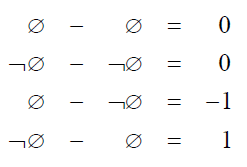
\includegraphics[width = 0.4\textwidth]{images/snapshotdiff.png}
		\end{center}
		\end{figure}
		\end{block}
	\end{frame}
	
\begin{frame}{Defining topological neighbors}
\begin{block}{}
Distance between any two relationships $r_A,r_B$ is given by: 
\begin{equation}
T_{r_A,r_B} = \sum\limits_{i=^0}^- \sum\limits_{j=^0}^-\left |M_A[i,j] - M_B[i,j]\right|
\end{equation}
\end{block}
\begin{block}{}
\begin{itemize}
\item It is the count of differences of empty/non empty entries of corresponding elements in the 9 intersections.
\item Shortest Nonzero distance between relations is 1
\item Spatial relations with the shortest non zero distance are considered topological neighbors. 
\end{itemize}
\end{block}
\end{frame}

\begin{frame}{Example 1}
\begin{block}{Are these relations neighbors according to the snapshot model?}
\begin{figure}
\begin{center}

\includegraphics[width = 0.7\textwidth]{images/example1snap.png}
\end{center}
\end{figure}
\end{block}
\end{frame}

\begin{frame}{Example 2}
\begin{block}{Another example... Are these relations topological neighbors ?}
\begin{figure}
\begin{center}

\includegraphics[width = 0.7\textwidth]{images/example2snap.png}
\end{center}
\end{figure}
\end{block}
\end{frame}

\begin{frame}{Conceptual neighborhoods derived from the snapshot model}
\begin{figure}
\begin{center}
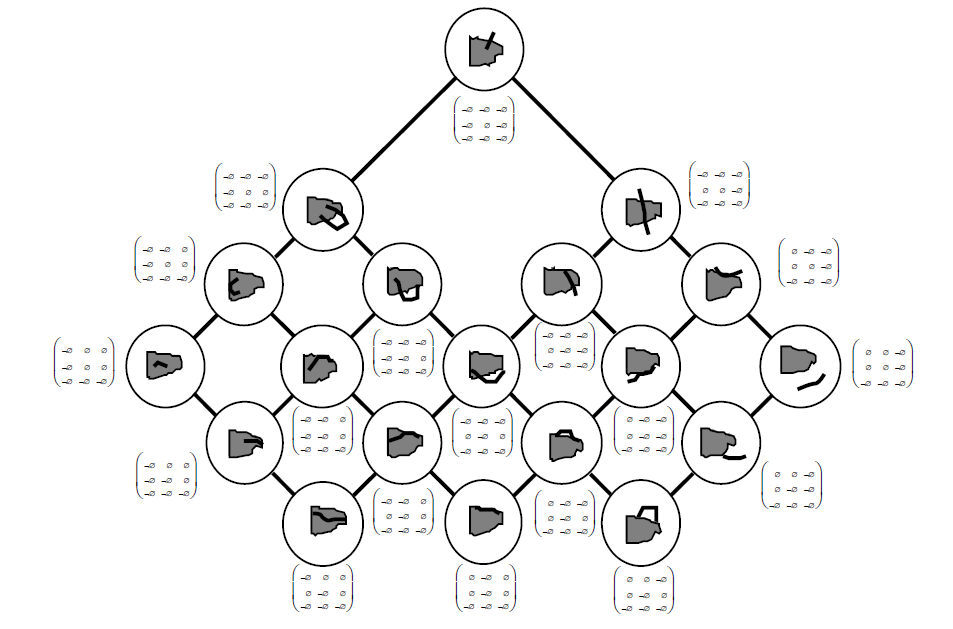
\includegraphics[width = \textwidth]{images/snapfull.png}
\end{center}
\end{figure}
\end{frame}